\documentclass{article}

%% SET MARGIN WIDTHS %%%%%%%%%%%%%%%%%%%%%%%%%%%%%%%%%%%%%%%%%%%%%%%%%%%%%%%%%%%

\setlength{\oddsidemargin}{-.3in}
\setlength{\evensidemargin}{-.3in}
\setlength{\textwidth}{6.9in}
\setlength{\topmargin}{-.9in}
\setlength{\textheight}{9.25in}

%% INCLUDE PACKAGES %%%%%%%%%%%%%%%%%%%%%%%%%%%%%%%%%%%%%%%%%%%%%%%%%%%%%%%%%%%%
\usepackage{amsmath}
\usepackage{amsfonts}
\usepackage{amssymb}
\usepackage{amsthm}
\usepackage{graphicx}
\usepackage{cite}
\usepackage{url}
\usepackage{adjustbox}
\usepackage{array}
\usepackage{array,multirow}
\usepackage{rotating}
\usepackage{wrapfig}
\usepackage{listings}
\usepackage[most]{tcolorbox}
\usepackage{inconsolata}
\usepackage{subfig}
\linespread{1.25}


\newcolumntype{R}[2]{%
    >{\adjustbox{angle=#1,lap=\width-(#2)}\bgroup}%
    l%
    <{\egroup}%
}
\newcommand*\rot{\multicolumn{1}{R{45}{1em}}}% no optional argument here, please!
\newcommand{\bs}{\(\blacksquare\)}
\renewcommand{\vec}[1]{\mathbf{#1}}


\newtcblisting[auto counter]{sexylisting}[2][]{	sharp corners,
												fonttitle=\bfseries,
												colframe=gray,
												listing only,
												listing options={basicstyle=\ttfamily, language=python},
												title= #2}

\title{Recombining Music using Similarity Scores}
\date{April 20, 2016}
\author{Ashton Baker}

\begin{document}

\maketitle

\section{Background}
\subsection{History of Algorithmic Music}
One of the first examples of algorithmic music was the dice game known as the \emph{Musikalisches Wurfelspiel}\cite{cope1996experiments}. The idea was to create a song, for which each measure of the song was chosen randomly from a pre-composed selection. So the first measure was chosen from the options for measure one, and so on. The earlies known example is Johann Kirnberger's \emph{Der allezeit fertige Polonoisen- und Menuettenkomponist}. Table 1 shows the table which is used to generate the six-measure polonaise. 

\begin{table}
\begin{center}
\begin{tabular}{c|c|c|c|c|c|c|}
    &  1 &   2&   3 &   4 &   5 &   6 \\ \hline
 2  & 70 &  34&  68 &  18 &  32 &  58 \\ \hline
 3  & 10 &  24&  50 &  46 &  14 &  26 \\ \hline
 4  & 42 &   6&  60 &   2 &  52 &  66 \\ \hline
 5  & 62 &   8&  36 &  12 &  16 &  38 \\ \hline
 6  & 44 &  56&  40 &  79 &  48 &  54 \\ \hline
 7  & 72 &  30&   4 &  28 &  22 &  64 \\ \hline
 8  &114 & 112& 126 &  87 &  89 &  88 \\ \hline
 9  &123 & 116& 137 & 110 &  91 &  98 \\ \hline
 10 &131 & 147& 143 & 113 & 101 & 115 \\ \hline
 11 &138 & 151& 118 & 124 & 141 & 127 \\ \hline
 12 &144 & 153& 146 & 128 & 150 & 154 \\ \hline
\end{tabular}
\end{center}
\caption{Table for \emph{Der allezeit fertige Polonoisen- und Menuettenkomponist}}
\end{table}

To use the table, one would simply roll two dice, and for the resulting roll, which can be from 2 to 12, there is a corresponding measure number. This measure was taken from a source, and used as the next measure of the polonaise. The measures had to be carefully composed so that each measure, when placed in a particular position, fulfills the same musical role as the others which are allowed to occupy that position. According to Cope, classical composers took these types of compositions quite seriously, using them not only as parlor games, but also as compositional tools and as a means to test their own understanding of musical rules and styles.

\subsection{David Cope}
The main inspiration for this project comes from the work of David Cope. Cope is one of the most successful algorithmic composers, and his Emmy Cope program has drawn interest from many different fields of research. Originally, I planned to recreate some of his algorithms, but it quickly became obvious that this would not be possible, as none of the source code is available, and his books are not sufficient to recreate his algorithms. So I will present here a general overview of Cope's system, and how it relates to my work. Cope presents the \emph{Musikalisches Wurfelspiel} as a starting point for his own work. For Cope, the next step is to quantitatively define sections of music, as well as the musical ``function'' of these sections. Here he develops the SPEAC system, to classify sections of music as either a Statement, Preparation, Extension, Antecedent, or Consequent, based on their context. Then, he is free to rearrange sections, needing only to transpose them so that they fit in contextually. This is only the first step of Cope's algorithm, but it gives the general sense of what he does.

My goal was to make music generation more assumption-free. I know much less about music theory than David Cope, and with that in mind I set out to design an algorithm for an automated sort of \emph{Musikalisches Wurfelspiel}, where the source measures could come from any other piece.

\section{Methods}
\subsection{Similarity Matrix}
The similarity matrix is developed as follows. Take two songs, \(A\) and \(B\), where \(A_m\) and \(B_m\) are the \(m^{th}\) note in the respective songs. Then define a matrix \(M\) such that \[M_{i, j} = (Pitch(A_i) - Pitch(B_j)) \mod 12.\] We'll call \(M\) the similarity matrix for \(A\) and \(B\). Each entry represents an interval between a note in \(A\) and a note in \(B\), adjusted mod 12 to simplify analysis (Though this would be a good assumption to reconsider with greater computational resources).

\begin{sexylisting}{Building a similarity matrix in Python}
def comparison_matrix(pattern_1, pattern_2):
    # Extract the pitch values of the ordered note on events
    a = [x.data[0] for x in flatten(pattern_1) if x.name == 'Note On']
    b = [x.data[0] for x in flatten(pattern_2) if x.name == 'Note On']

    matrix = []
    for x in b:
        new_line = []
        for y in a:
            new_line.append((x - y) % 12)
        matrix.append(new_line)
    return matrix
\end{sexylisting}

The similarity matrix is demonstrated in Figure \ref{fig:fugue-matrix}. This shows Bach's Fugue in G Major (BWV 541) compared with itself, with each color representing a different interval from 0 to 11. Both a full view and a close-up are shown. In the full view, the different sections of the piece are visible as they create the stripes in a sort of plaid pattern. In the close view, which covers about the first 150 notes of the piece, we can see the diagonal is blue, representing zero. This makes sense, since \(M_{i,i} = Pitch(A_i) - Pitch(A_i) = 0\). It is difficult to draw many conclusions from this multi-colored plot, but it is interesting to play with using the \texttt{music.explore()} function.

\begin{figure}[h]
\begin{center}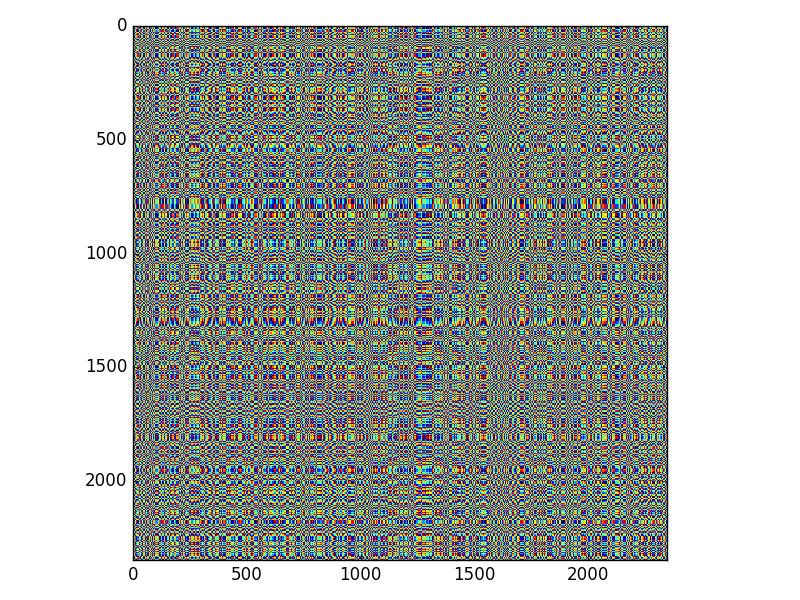
\includegraphics[width=0.5\textwidth]{figure_1.png}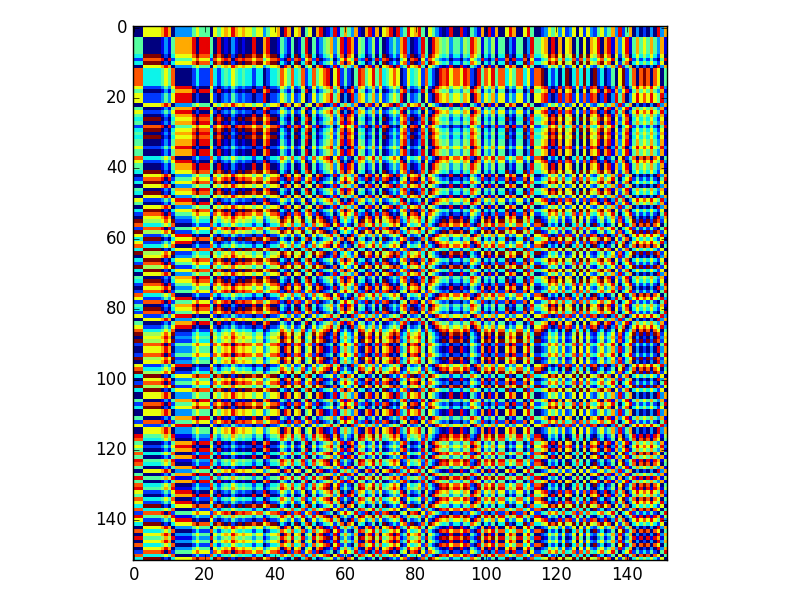
\includegraphics[width=0.5\textwidth]{figure_2.png}
\end{center}\caption{Self-similarity demonstrated with a Bach fugue} \label{fig:fugue-matrix}
\end{figure}

\subsection{Filtering the Similarity Matrix}
Looking at all the intervals at once isn't particularly illuminating. A good next step is to filter the matrix for only a particular interval. Then we can look for diagonal runs that represent similar sections. We have already simplified our work by reducing the number of possible intervals to 12. Figure 2 shows a typical result of this type of filtering, using a search for intervals equal to 7.

\begin{figure}[h]
\begin{center}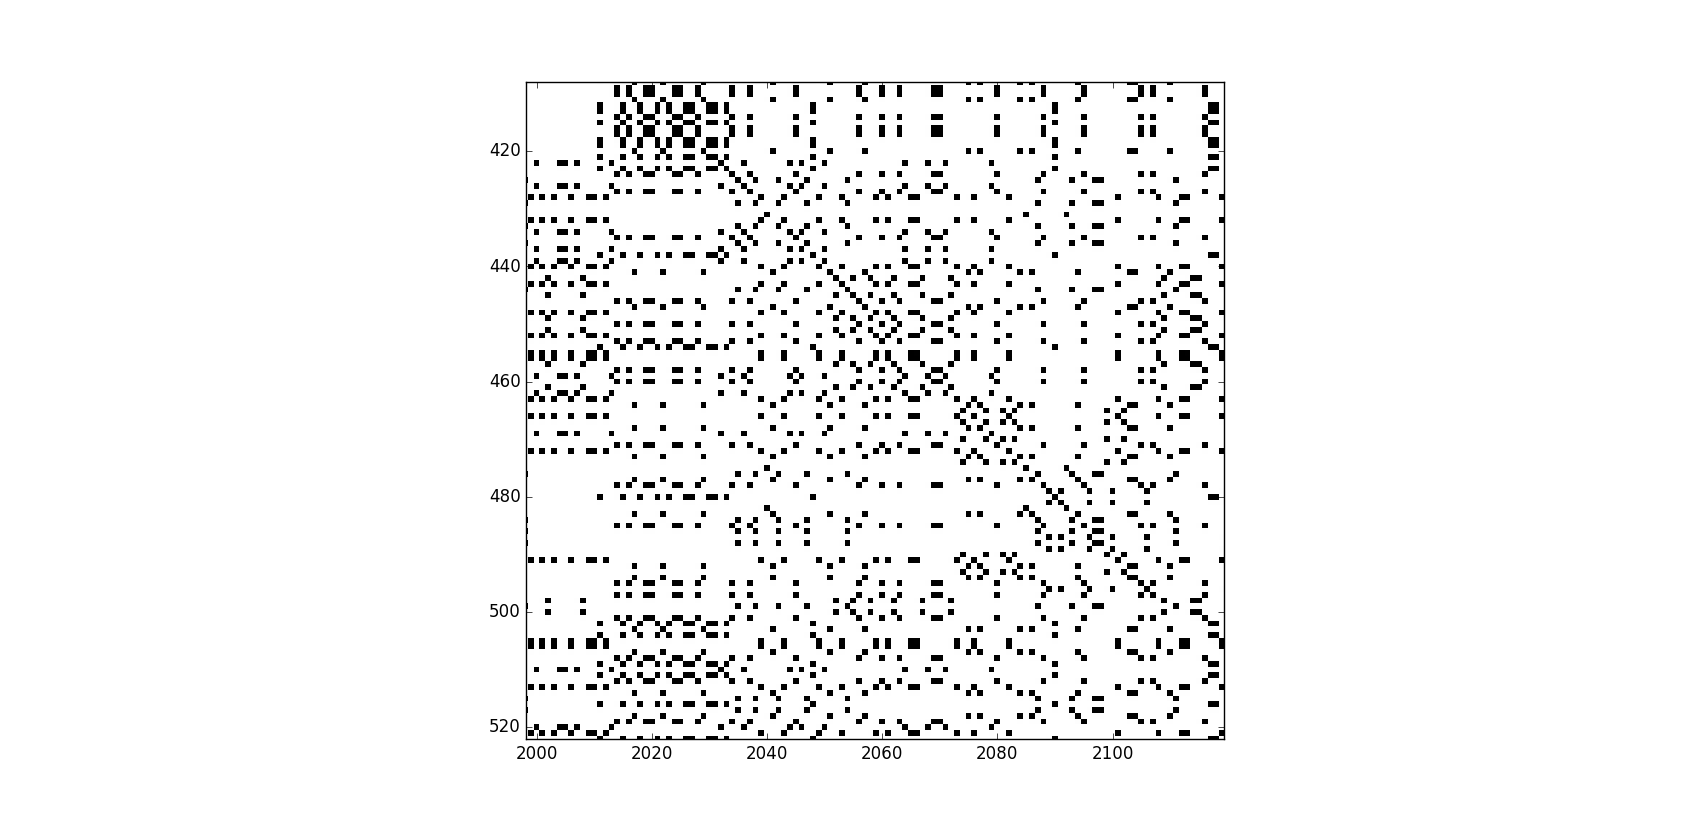
\includegraphics[width=0.7\textwidth]{figure_4.png}
\end{center}\caption{Filtering by a single interval} \label{fig:single-interval}
\end{figure}

The organization of the elements into a diagonal line indicates that the sections of the song which lie on the margins are similar to each other, but transposed by 7. This allows us to quickly visually identify repeated sections in pieces. This gives us our first concrete results. The next step is to automate the process.

\subsection{Filtering for Diagonal Shapes}
The simplest way to identify runs is to only allow diagonal runs. Then we can determine the length of each run by just counting down and right until we reach the end. If the run is long enough, it is saved. Otherwise, it is cleared from the board. Figure \ref{fig:diag-filtering} shows this type of filtering. The long perfect diagonal on the right is preserved, as well as an area before it that appears to have a few insertions and deletions. Also, this method does an excellent job of filtering out background noise. One disadvantage is that the method only preserves perfect runs. The occasional insertion or deletion is okay, as long as the run of notes in between is long enough that it doesn't fall under the threshold. In genomics, indels don't tend to happen at small, repeated intervals, but in music, it happens all the time. Figure \ref{fig:indel-example} gives an example of repeated insertions/deletions, which can happen when a composer doubles the tempo, or plays variations on a theme. 

\begin{figure}[h]
\begin{center}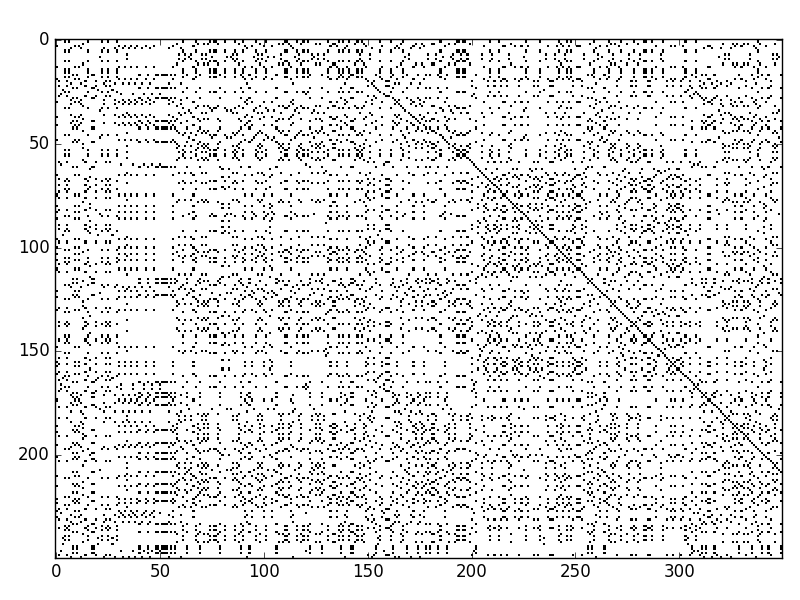
\includegraphics[width=0.5\textwidth]{easybefore.png}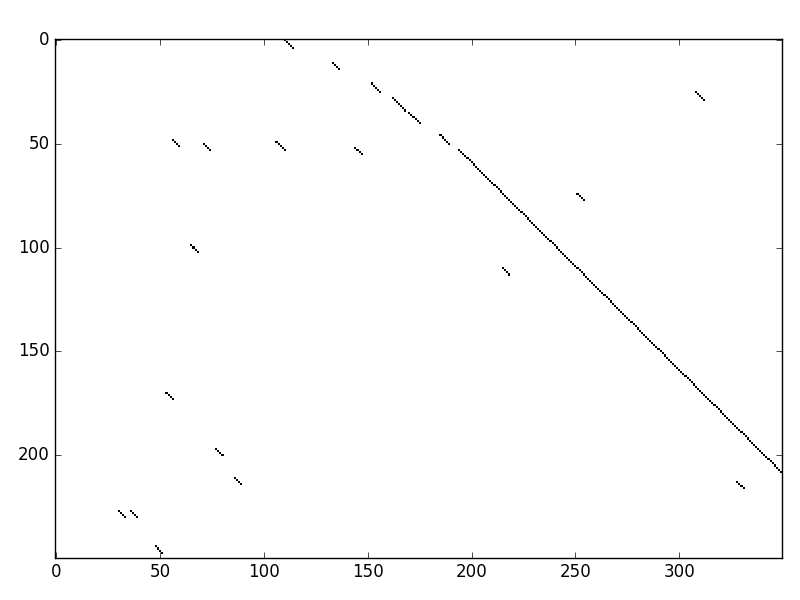
\includegraphics[width=0.5\textwidth]{easyafter.png}
\end{center}\caption{Before and after filtering for 3-diagonal runs} \label{fig:diag-filtering}
\end{figure}

Also shown is the comparison matrix for intervals of size zero. The gaps in the path would cause the path to be removed as background noise by our current algorithm, so we will develop a new one which can capture this flexibility to insertions and deletions. 

\begin{figure}[h]
  \centering
  \raisebox{-0.5\height}{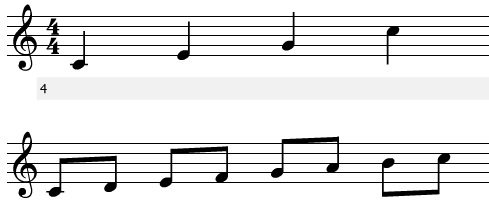
\includegraphics[height=1.25in]{example.png}}
  \hspace*{.2in}
  \raisebox{-0.5\height}{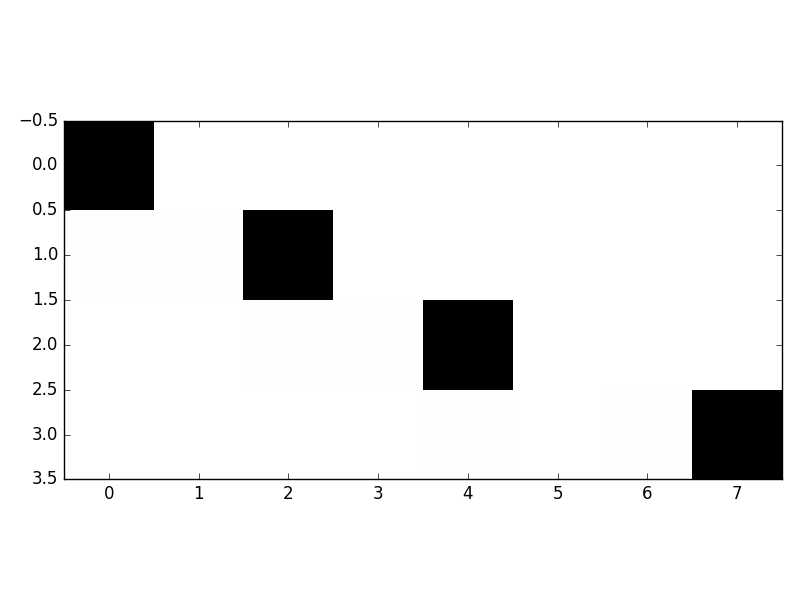
\includegraphics[height=1.75in]{example2.png}}
  \caption{Musical example of insertion/deletions} \label{fig:indel-example}
\end{figure}

The algorithm begins with a series of allowable steps. I decided to allow for up to 2 insertions or deletions at a time. Thus, we could jump from \((0, 0)\) to any of \((1, 1)\), \((1, 2)\), \((1, 3)\), \((2, 1)\), \((2, 2)\), or \((3, 1)\). To give an overview of the algorithm, we will create a tree at each black dot, with branches extending to any of the allowable spaces which also contain a black dot. At each iteration, a branch will only be extended to a grid point if a longer branch has not already reached there. This is done to prevent overlapping paths, and because it always favors deleting a shorter path over a longer one. Next, each point which serves as a leaf of one of the many trees can follow a unique path back to its root. After reaching the root, if this is the longest path to reach the root so far, we sign the name of the leaf, as well as the length of the path on the root, so that if we reach the same root again via a shorter path, we know to throw that path out.

This explanation doesn't sacrifice much in terms of accuracy. The technical details mostly involve implementing a node structure in Python, and are probably best explained as comments alongside the code. So I will direct the interested reader to github.com/ashtonbaker/mth-563-final-project, specifically the \texttt{identify runs()} function in the \texttt{music.py} module.

Figure \ref{fig:worm-filtering} shows the results of this filter. Only runs of length 10 or greater are shown. This method captures the long diagonal much better, as a single piece. And additionally, the algorithm keeps a record of all the runs it finds, so instead of a fractured collection of dots, we have information that we can use to determine similarity. 
\begin{figure}[h]
\begin{center}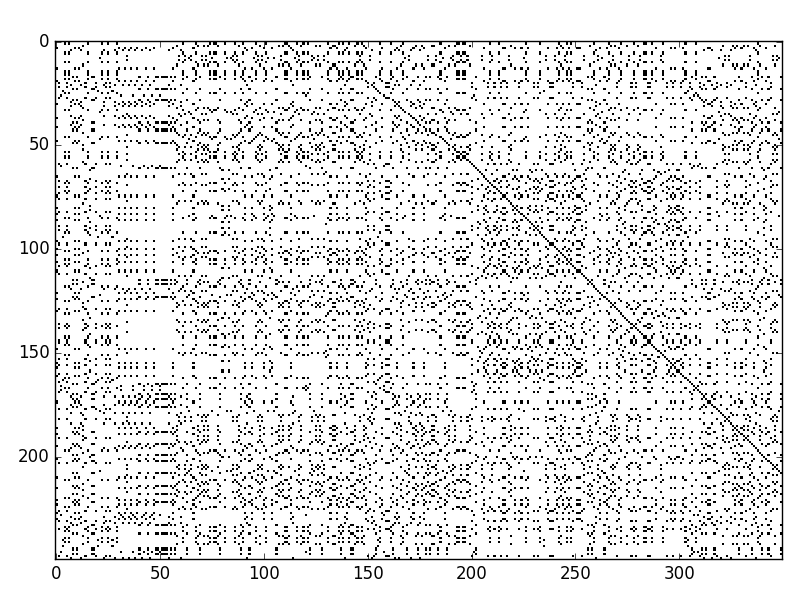
\includegraphics[width=0.5\textwidth]{before.png}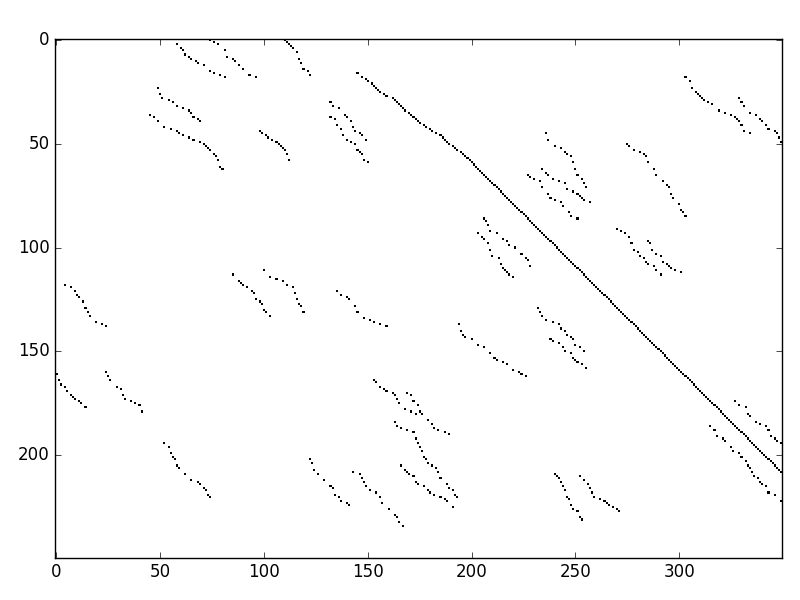
\includegraphics[width=0.5\textwidth]{after.png}
\end{center}\caption{Before and after run-filtering} \label{fig:worm-filtering}
\end{figure}
Compared to Figure \ref{fig:diag-filtering}, there are many more long runs. Comparing the filtered version to the original, most of these runs are not detectable visually, and instead appear to be a result of repeated linear artifacts in the original. This is a consequence of our generous allowance of up to 2 insertions or deletions. Generally, more allowable steps will lead to a noisier background and more long runs.

The followin code box shows a summary of the runs detected for BWV 529-1 and BWV 541-2. These are the longest runs associated with each transposition degree. So notes 692 to 714 of Track A match notes 1073 to 1092 of Track B. This gives us a place to start with more subjective analysis.

\begin{sexylisting}{Similarity Summary for two pieces}
Track A: bwv529-1.mid
Track B: bwv0541f.mid

A 692 to 714 and B 1073 to 1092: 14 notes (63.6 percent similar), trans -6
A 365 to 432 and B 2230 to 2293: 35 notes (52.2 percent similar), trans -5
A 653 to 699 and B 1408 to 1455: 27 notes (57.4 percent similar), trans -4
A 1783 to 1822 and B 1880 to 1926: 25 notes (54.3 percent similar), trans -3
A 695 to 786 and B 1206 to 1282: 46 notes (50.5 percent similar), trans -2
A 1003 to 1032 and B 1927 to 1950: 16 notes (55.1 percent similar), transp -1
A 185 to 251 and B 2021 to 2091: 40 notes (57.1 percent similar), trans 0
A 1337 to 1364 and B 757 to 782: 15 notes (55.5 percent similar), trans 6
A 2278 to 2345 and B 2230 to 2293: 35 notes (52.2 percent similar), trans 7
A 2567 to 2613 and B 1408 to 1455: 27 notes (57.4 percent similar), trans 8
A 1691 to 1726 and B 17 to 53: 22 notes (61.1 percent similar), trans 9
A 2609 to 2700 and B 1206 to 1282: 46 notes (50.5 percent similar), trans 10
A 2579 to 2597 and B 1075 to 1099: 12 notes (50.0 percent similar), trans 11
\end{sexylisting}

\subsection{Similarity Scores}
Intuitively, we should be able to use these diagonal runs to say something about the similarity of two pieces. For example, if the longest run is the length of one of the pieces, then one piece is a subset of the other, or matches completely. On the other hand, if we don't find any diagonal runs, then we could give a similarity score of zero. But what about the much more common cases in between? Figure \ref{fig:random-filtering} shows the difficulty. This is a comparison of intervals of distance 0, for Bach's Fugue in G and Trio Sonata 5 Mvt 1. There are several diagonal runs, and this density is reflective of the entire grid. So how should we calculate the similarity in this case?

\begin{figure}[h]
\begin{center}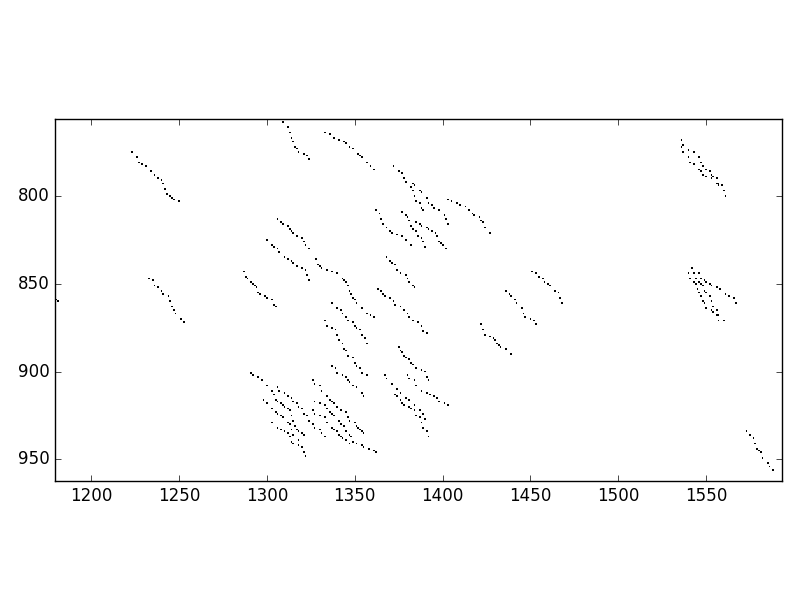
\includegraphics[width=0.5\textwidth]{random.png}
\end{center}\caption{Comparison of Bach's Fugue in G (BWV 541) and Trio Sonata 5 Mvt 1} \label{fig:random-filtering}
\end{figure}

Ideally, I think the solution would go something like this. We should, first of all, choose runs so that they do not overlap in either the x-direction or the y-direction. The runs should be chosen so that they leave as few blank spaces as possible. Then, we could calculate the portion of columns with a black dot, or the portion of rows. This would be the similarity score. I couldn't find an efficient algorithm for this, and I suspect it is in some way equivalent to the maximum coverage problem, which is NP-hard.

A greedy algorithm for approximating this is probably the best option. So we order the runs from longest to shortest, and repeatedly select the longest run which does not overlap with any of the already-chosen runs. This is a very efficient method, and gives us a good approximation to the ideal. Since a similarity score is sort of a nebulous concept anyway, this seems to be a valid approach.

\section{Results}
\subsection{Music Generation}
Actually generating music turned out to be incredibly difficult. The plan was to break up a MIDI song measure-by-measure, and to compare each measure with measures from other songs. Then, measures in the original song would be swapped for measures from other songs, with the probability of choosing a measure weighted by its similarity score to the measure being swapped out. I actually have all of the software tools to do this, as described in the next subsection, but I've met with two problems. First, MIDI files do not encode measure numbers, so these must be manually calculated. However, I've found that MIDI files from different sources use different conventions as to locations of tempo and time signature events, and so on. Secondly, I haven't actually been able to assemble a MIDI file with the package I've been using. I am interfacing with MIDI through the \texttt{python-midi} package at \texttt{https://github.com/vishnubob/python-midi}, and there is a bug that sometimes affects tick numbers when assembling MIDI files. I bit off more than I could chew, code-wise. However, the tools produced for this project will make this a very simple task for anyone who can break MIDI files into measures.

\subsection{Python tools for MIDI analysis}
In the course of investigating this project, I developed some tools which have considerable power to analyze and compare MIDI files. The music.py package contains the following functions
\begin{description}
\item[comparison matrix] Takes two MIDI patterns and returns a similarity matrix

\item[find intervals] Filters a similarity matrix for a single interval

\item[flatten] Combines all MIDI events in a song into one track, automatically handling relative tick values

\item[explore] Uses matplotlib to show an interactive similarity matrix, filtered or unfiltered.

\item[note range] Takes a MIDI pattern and outputs a range of notes, in chronological order.

\item[identify runs] Use to detect every diagonal run beyond a given threshols, and of a particular interval value. Can be configured to use different steps when calculating acceptable runs. This function also determines the transposition magnitude and direction that should be given to each run in order to best align it with Track A.

\item[summarize similarity] Searches all the diagonal runs between two songs, and summarizes the longest ones in plain English. Helpful to begin investigaion of similar sequences between songs.

\item[similarity score] Returns a semi-optimized similarity score for two MIDI tracks. Ranges from 0 (least similar) to 1 (identical).
\end{description}

\subsection{Similarity Scores for Bach Pieces}
Table \ref{tab:insurgency_outcomes} shows some similarity scores for various Bach pieces. These take a long time to calculate, even using the Bioinformatics department server, so I limited myself to a few, as a proof-of-concept. It is perhaps surprising that the scores are so high, but we used very lenient instructions for calculating runs, and we sought to maximize coverage while calculating scores, so it is perhaps not \emph{too} surprising. The scores are all very close, so if we take this at face value, then a small difference in score could mean a large difference in actual content. The most similar pieces are BWV 529-1 and BWV 541 - Fugue, which makes sense, as they are both upbeat major-key songs. 

In terms of future work, we could also assign directionality to this network, according to when the piece was written. Then, we would see how ideas flow over time, and we could do network analysis to determine ``neighborhoods'' of composers, or of pieces, and the most central or important composers.

\begin{table}[h]
\centering
\resizebox{0.5 \columnwidth}{!}{%
\begin{tabular}{c r| c|c|c|c|c|}
\\
& \multicolumn{1}{ c }{} & \multicolumn{5}{c}{ \null } \\
& \multicolumn{1}{ c }{} &
\rot{BWV 529-1}&
\rot{BWV 529-2} &
\rot{BWV 529-3} &
\rot{BWV 541-P} &
\rot{BWV 541-F} \\ \cline{3-7}
\multirow{16}{*}{ \null }
&BWV 529-1 & 1.000 & 0.448 & 0.523 & 0.498 & 0.576 \\ \cline{3-7}
&BWV 529-2 & 0.448 & 1.000 & 0.465 & 0.512 & 0.461 \\ \cline{3-7}
&BWV 529-3 & 0.523 & 0.465 & 1.000 & 0.587 & 0.624 \\ \cline{3-7}
&BWV 541-P & 0.498 & 0.572 & 0.587 & 1.000 & 0.587 \\ \cline{3-7}
&BWV 541-F & 0.576 & 0.461 & 0.624 & 0.589 & 1.000 \\ \cline{3-7}
\end{tabular}%
}\caption{Similarity scores for various Bach pieces}\label{tab:insurgency_outcomes}
\end{table}

\nocite{*}
\bibliography{bibliography.bib}{}
\bibliographystyle{plain}

\end{document}
